\section{Technologien}
In diesem Kapitel soll alles zum Thema Technologien zusammengefasst sein.
Zusätzlich sollen Schaubilder und Diagramme das Verständies für die Technologien erleichtern.
Sowie Beschreibungen und Erklärungen zu der Wahl der einzelnen Technologien.

\subsection{Entscheidung für die Technologien}
Bei der Wahl der Technologien haben wir nach Möglichkeit LTS Versionen gesucht.
Damit wir eine Applikation erstellen können, die für lange Zeit Sicherheitsupdates
bekommt. Zusätzlich haben wir als Ziel, dass die Software als ingesamtes Paket sehr lange
stabil läuft und dadurch Ausfälle minimiert werden.

\subsection{Technologie Versionen}
Hier sollen die einzelnen Technologien im Einzelnen beschrieben werden.
Sowie ihre geplante Funktion in unserem Projekt.

\begin{table}[H]
    \begin{center}
        \begin{tabular}{|c|c|}
            \hline
            
\includegraphics[width=0.15\textwidth]{bilder/technologien/NodeJS.png}    &
            \multirow[c]{1}[1]{*}[30pt]{Node.js 16.13.0 LTS}                            \\
            \hline
            
\includegraphics[width=0.15\textwidth]{bilder/technologien/Angular.png}   &
            \multirow[c]{1}[1]{*}[30pt]{Angular 13.0.1}                                 \\
            \hline
            
\includegraphics[width=0.15\textwidth]{bilder/technologien/Socket.io.png} &
            \multirow[c]{1}[1]{*}[30pt]{Socket.io 4.3.2}                                \\
            \hline
            
\includegraphics[width=0.15\textwidth]{bilder/technologien/mongoDB.png}   &
            \multirow[c]{1}[1]{*}[30pt]{MongoDB Community Edition 5.0.3}                \\
            \hline
            
\includegraphics[width=0.15\textwidth]{bilder/technologien/KeyCloak.png}  &
            \multirow[c]{1}[1]{*}[30pt]{KeyCloak 15.0.2}                                \\
            \hline
            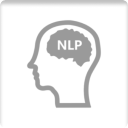
\includegraphics[width=0.15\textwidth]{bilder/technologien/NLP.png}       &
            \multirow[c]{1}[1]{*}[30pt]{NLP.js 4.22.2 (optional)}                       \\
            \hline
        \end{tabular}
        \caption{Technologie Liste}
        \label{tab:Technologie Liste}
    \end{center}
\end{table}


\subsubsection{Node.js 16.13.0 LTS}
Als Basis für Angular, den Chatbot und Keycloak nutzen wir eine LTS Version von Node.js.
Auf dem Node.js Server verwenden wir zusätzlich die Express Erweiterung,
um eine Kommunikation zu den Servern herstellen zu können.
Für uns war sehr wichtig, dass wir eine sehr stabile Basis für die Anwendung,
die wir entwickeln haben.
Deswegen haben wir uns ebenfalls informiert, ob alle geplanten oder in Frage kommenden Technologien mit der LTS Version kompatibel sind.
Nach unserem derzeitigen Stand empfehlen die Entwickler der Bibliotheken und Framworks eine LTS Version von Node.js zu verwenden.
Bildquelle:\cite{nodejsicon}


\subsubsection{Angular 13.0.1}
Wir verwenden Angular für die Frontend-Entwicklung.
Angular ist die Basis, um das Chat- und das Admin-Interface zu erstellen.
Um unsere UIs noch effektiver zu gestalten werden wir vereinzelt auf Angular Material zurückgreifen.
Dort gibt es zu häufig genutzten UI Komponenten "Code Snippets", die ausführlich getestet wurden.
Bildquelle:\cite{angularicon}

\subsubsection{Socket.io 4.3.2}
In unserem Projekt nutzen wir Socket.io, um eine bidirektionale Kommunikaton zwischen dem Bot und
der Benutzeroberfläche herzustellen.
Es ermöglicht uns, dass ein User mit dem Chatbot ohne merkbare Verzögerung chatten kann.
Bildquelle:\cite{socketioicon}

\subsubsection{MongoDB Community Edition 5.0.3}
Wir haben uns für die Datenbank mongoDB entschieden, da es ein sehr einfaches Datenbank Modell bereitstellt.
MongoDB ist eine NoSql Datenbank wodurch auch der Verwaltungsaufwand der Datenbank minimiert wird.
In der Datenbank wird der Korpus des Chatbots gespeichert.
Bildquelle:\cite{mongodbicon}

\subsubsection{KeyCloak 15.0.2}
In unserem Projekt verwenden wir KeyCloak, damit sich der Admin sicher in das Admin-Webinterface einloggen kann.
Zusätzlich werden wir das Shibboleth Single-Sign-On Verfahren von der Hochschule integrieren.
Damit Hochschulangehörige die Möglichkeit haben mit ihrem Hochschul Account sich einloggen zu können.
Dadurch können wir zusätzlichbegrenzen welche Personengruppen auf welche Daten Zugriff haben.
Bildquelle:\cite{keycloakicon}

\subsubsection{RegEx}
Wir haben in unserem Projekt anfangs aus Sicherheitsgründen RegEx eingeplant.
Um ein Scheitern des Projektes zu verhindern, falls NLP.js sich nicht in unser Projekt integrieren lassen sollte.
Somit der Chatbot dennoch Begriffe und Sätze verstehen kann.
Nach unserem derzeitigen Stand brauchen wir nicht auf eine RegEx Implementation zurückzugreifen,
da NLP.js sich sehr gut in unser Projekt integrieren lässt.
Bildquelle:\cite{regexicon}

\subsubsection{NLP.js 4.22.2 (optional)}
Damit wir NLP.js nutzen können benötigen wir eine LTS Version von Node.js.
Diese Begrenzung haben wir zusätzlich in die Technologie Entscheidung einbezogen.
Wir haben den NLP.js ausführlich getestet und werden es als Basis für den Chatbot verwenden.
Indem NLP.js ab der Version 4 und höher modular ist. Wird uns ermöglicht leichter eigene Module/Plugins
für das Framework zu schreiben.
Dadurch können wir einen ChatBot mit verbesserter Spracherkennung gestalten.
Bildquelle:\cite{nlpicon}